\documentclass[10pt,a4paper]{article}
\usepackage[latin1]{inputenc}
\usepackage[dutch]{babel}
\usepackage{amsmath}
\usepackage{amsfonts}
\usepackage{amssymb}
\usepackage{graphicx}
\usepackage{listings}
\author{Ruben Van Assche - S0122623}
\title{Wetenschappelijk Programmeren: Orthagonale Baisifuncties - Oefening 1}
\begin{document}
\maketitle
\section{Opgave}
In deze opgave moest een functie $e^{-x}*sin(\pi *x)$ benaderd worden door een least squares approximatie van graad 4 waarbij de datapunten bepaald worden door de nulpunten van het Chebychev Polynoom van graad 11. Dit op het interval [-1, 1]. Vervolgens moest een kleinste kwadraten trigoniometrische benadering bepaald worden van dezelfde vergelijking op het interval [-$\pi$, $\pi$]. Waarbij de nulpunten gegeven worden door $- \pi + 2 \pi i/11$. 

\section{Chebychev}
Eerst moeten we de nulpunten van $T_{11}(x)$ berkenen, dit kan door: $$cos(\frac{(2j-1)*\pi}{2*i})$$ hierbij is $i = 11$ de graad van het chebychev polynoom en loopt j van 1 tot 11. Voor deze elf punten rekenen we vervolgens de y waarden uit d.m.v. de functie $e^{-x}*sin(\pi *x)$. 
\newline
Hierna is het nog een kwestie van d.m.v.\detokenize{gsl_multifit_linear} het stelsel op te lossen: 
\newline
$$
\begin{bmatrix}
x_{1}^{0} & x_{1}^{1}  & x_{1}^{2}  & x_{1}^{3}  & x_{1}^{4}\\ 
 \vdots & \vdots  & \vdots  &\vdots   & \vdots \\ 
x_{10}^{0} &  x_{10}^{1} & x_{10}^{2}  & x_{10}^{3}  & x_{10}^{4}
\end{bmatrix}
\begin{bmatrix}
\lambda_{0}\\ 
\vdots \\
\lambda_{4}\\ 
\end{bmatrix}
=
\begin{bmatrix}
y_{0}\\ 
\vdots \\
y_{10}\\
\end{bmatrix}
$$
We verkrijgen hierdoor een approximatie voor $\lambda_{0}, ..., \lambda_{4}$. Deze worden ingevuld in g(x) en vervolgens verkijgen we:
$$g(x) = \lambda_{0} + \lambda_{1}*x + \lambda_{2}*x^{2} + \lambda_{3}*x^{3} + \lambda_{4}*x^{4}$$
In het geval van $e^{-x}*sin(\pi *x)$ wordt g(x): 
$$g(x) = -0.042053 + 2.9601*x - 2.3619*x^{2} - 3.0056^{3} + 2.4429*x^{4}$$
Vervolgens plotten we f(x) (BasicPoints1.dat) en g(x) (ChebyChevLeastSquares.dat):
\newline
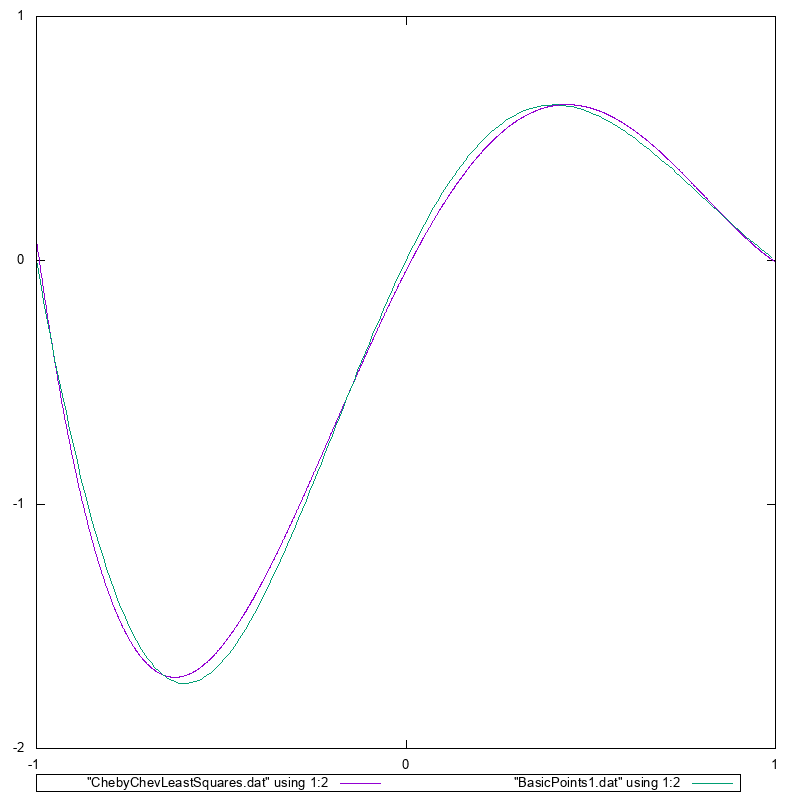
\includegraphics[scale=0.7]{ChebyChevLeastSquares.png}
\newline
We zien dat dit een mooie approximatie is voor f(x).

\subsection{Orthogonaliteit}
Pas vrij laat besefte ik dat deze opgave ook op te lossen was d.m.v. de orthogonaliteit van Chebychev functies. Hierbij worden de $\lambda_{i}$niet meer berekend op basis van het oplossen van een stelsel maar d.m.v. een simpele vergelijking: 
$$ \lambda_{j} = \frac{\sum^{n}_{i = 1}T_{j-1}(x_{i})*y_{i}}{m/2}$$
Hierbij is n = 11 en m = 5. Helaas verkreeg ik nooit een goed resultaat en heb ik de berkening achterwege gelaten. Mijn 2 pogingen staan nog wel in de broncode met functienamen: generateChebychevLeastSquares2, generateChebychevLeastSquares3 in het bestand Trio.cpp.
 
\section{Trigoniometrisch}
Om een trigoniometrische least squares approximatie te verkrijegen is het niet verreist dat een complexe matrix moet opgelost worden. D.m.v. orthagonale basisfuncties weten we inmiddels dat $g(x) = \frac{a_{0}}{2}+a_{1}*cos(x)+b_{1}*cos(x)+b_{2}*cos(2x)+a_{2}*cos(2x)$. Hierbij is $g(x)$ de benaderde functie en geldt dit voor graad 2. Nu rest ons enkel nog $a_{0}, a_{1}, a_{2}, b_{1}, b_{2}$ te berekenen.
$$a_{j} =  \frac{2}{11}\sum_{k = 0}^{10}y_{k}*cos(j*x_{k})$$
$$b_{j} =  \frac{2}{11}\sum_{k = 0}^{10}y_{k}*sin(j*x_{k})$$
Deze $a_{i}$ en $b_{i}$ zijn zeer makkelijk te berekenen en voor de opgave komen we dan volgende waarden uit:
\newline
\begin{tabular}{lll}
\textbf{i} & \textbf{a}               & \textbf{b}             \\
\textbf{0} & -0.029835274480727081575 & 0                      \\
\textbf{1} & 0.047513231220430197921  & 0.73378196483313440357 \\
\textbf{2} & 0.1349790515049160144    & -1.9614672973839133441
\end{tabular}
Deze worden dan ingevuld in $g(x) = \frac{a_{0}}{2}+a_{1}*cos(x)+b_{1}*cos(x)+b_{2}*cos(2x)+a_{2}*cos(2x)$ en onze approximatie is klaar!
\newline
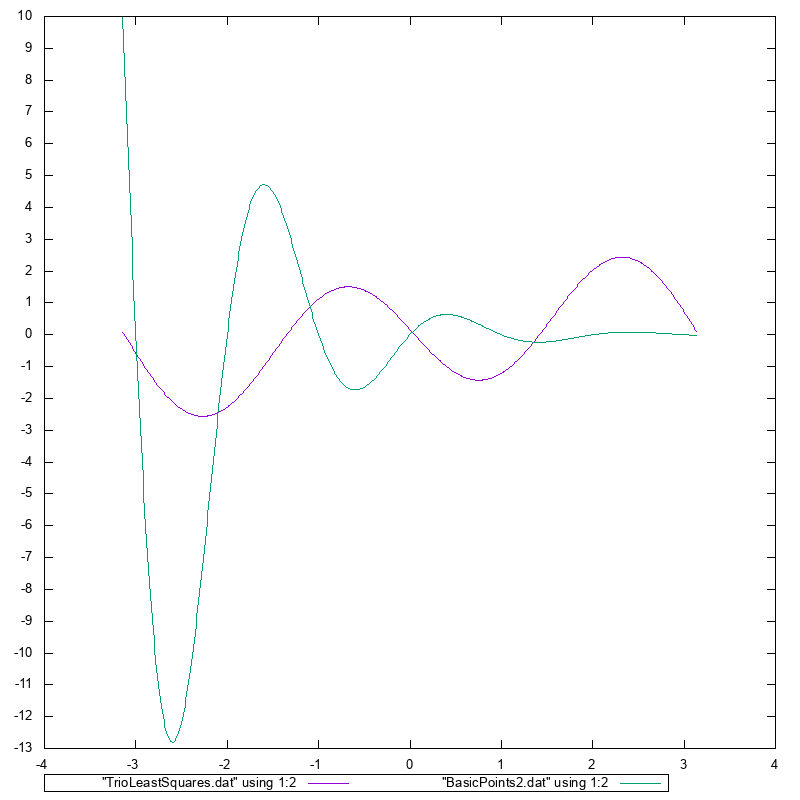
\includegraphics[scale=0.7]{TrioLeastSquares}
Het eerste wat opvalt is dat dit geen goede approximatie is, de grafiek volgt de originele curve wel wat(dalen en stijgen) maar komt zeker niet in de buurt van een goede approximatie. Eerst dacht ik dat er een fout in mijn code zat maar andere functies zoals $sin(x), cos(x) en x^{2}$ hebben wel goede approximaties. Waarschijnlijk kan het verhogen van de graad helpen(weliswaar oppassen dat deze niet groot wordt $n > 2m+1$) of datapunten kiezen op andere plaatsen.

\section{Code}
\textbf{Util.cpp - Wat basiscode voor beide opgaven}
\lstinputlisting{../util.cpp}
\textbf{Chebychev.cpp - Code voor de Chebychev opgave}
\lstinputlisting{../chebychev.cpp}
\textbf{Trio.cpp - Code voor de trigoniometrische opgave}
\lstinputlisting{../trio.cpp}

\end{document}